\section{Benutzer Interface}



Konzepte, die haupts�chlich dazu dienen mit dem Spieler zu interagieren und sehr abh�ngig von seinen Entscheidungen sind.


\subsubsection{Richtungsangabe}
\begin{wrapfigure}{r}{0.4\textwidth}
  \begin{center}
    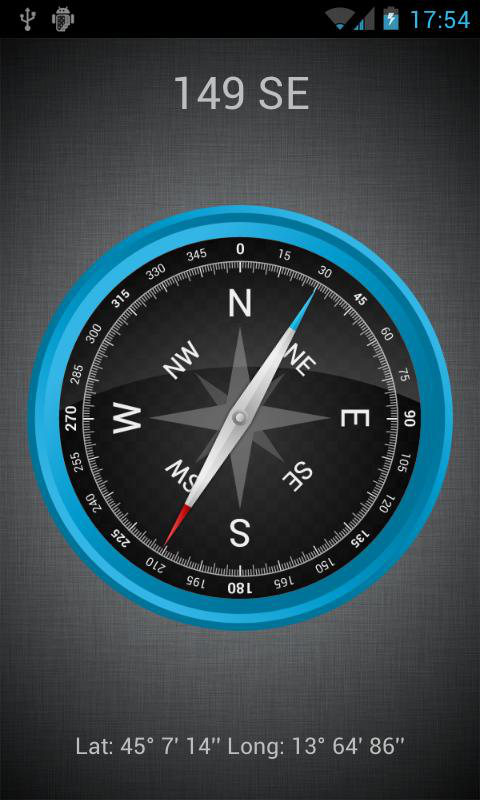
\includegraphics[width=0.3\textwidth]{3-Spielkonzepte/3-2-Benutzer_Interface/kompass.png}
     \caption{Integrierter Kompass unter Android
	(Quelle: \url{https://lh6.ggpht.com/tQTY2Itaq9YtG8CZh8RA0N7sekCbURqBG5ZcpV6_u2no8Y8ezVIEibB4udVNFLzYKA\%3Dh900})
		}
  \end{center}
\end{wrapfigure}

Eine Richtungsangabe kann eine Karte ersetzen. Sei es um bei �Capture the Flag� die Richtung der Fahne des Gegners anzuzeigen oder f�r �Snake� das n�chste einzusammelnde Item. Auch ein Kompass dient als Richtungsangabe und findet beim oben erw�hnten "`Geocaching"' teilweise seinen Einsatz.
\newline
Die technischen L�sungen f�r eine Richtungsangabe sind unter Positionsermittlung (s. \ref{positionsermittlung}), GUI (s. \ref{gui}) und Andere Sensorik (s. \ref{sensorik}) zu finden.

\subsubsection{Akustische und haptische Orientierungshilfen}

Akustische oder haptische Signale k�nnen ebenso Hinweise auf in der N�he
befindliche Interessengebiete geben (z.B. ert�nen eines Signals oder Vibration beim Erreichen eines bestimmtem Umkreises eines Items). 
Akustische oder haptische Signale k�nnen aber auch als Best�tigung eingesetzt
werden, wenn z.B. etwas eingesammelt wurde.
\newline
Zur Best�tigung einer Kollision wird die Kollisionsabfrage (s. \ref{kollisionsabfrage}) ben�tigt. Unter Andere Sensorik (s. \ref{sensorik}) ist mehr zu akustischen und haptischen Signalen zu finden.


\subsubsection{Geschwindigkeitsmessung}
Um das Spielgeschehen besser zu kontrollieren zu k�nnen, kann eine Messung der
Geschwindigkeit von Vorteil sein. M�chten wir z.B. bei Capture the Flag dem Fahnentr�ger nicht erlauben eine gewisse Geschwindigkeit zu �berschreiten, ist eine Geschwindigkeitsmessung unabdingbar.
\newline
Um diese umsetzen zu k�nnen wird Positionsermittlung (s. \ref{positionsermittlung}), Server-Client-Kommunikation (s. \ref{kommunikation}) und Andere Sensorik (s. \ref{sensorik}) ben�tigt.


\subsubsection{Mensch-Maschine-Kommunikation}\label{sec:mensch-maschine-kommunikation}
Das komplette Spielgeschehen lebt von der Integrierung der mobilen Endger�ten und der Kommunikation zwischen Mensch und Ger�t. Wird auf dem Endger�t eine Richtungsanzeige eingeblendet, muss der Spieler insofern reagieren, dass er sich in die richtige Richtung dreht. Wenn er etwas einsammeln m�chte, kann es erforderlich sein, dass ein Button gedr�ckt wird.
\newline
Daf�r ben�tigt wird die GUI (s. \ref{gui}) bzw. die Kartendarstellung (s. \ref{kartendarstellung}).